% !TEX root = ../dissertacao.tex
\chapter{Conceitos Fundamentais}
\label{cap:conceitos_fundamentais}

\section{Arquitetura do Sistema de Memória}
\label{sec:conceitosFundamentaisArquitetura}
% conceitos em arquitetura de computadores
%     -- niveis de cache
%     -- miss
%     -- hit

A arquitetura de memória de computadores modernos é tipicamente hierárquica, como mostrado na Figura~\ref{fig:memoryHierarchy}, onde os níveis mais baixos na hierarquia (disco rígido e memória principal) têm maior maior capacidade de armazenamento, mas apresentam maior latência.
Por outro lado, os níveis mais altos (memória \textit{cache} e registradores da CPU) são rápidos, mas possuem capacidade de armazenamento limitada.
Quando um determinado programa precisa de um dado, mas o mesmo não se encontra nos registradores da CPU, será realizada uma busca por este dado nos níveis mais altos da hierarquia da memória, iniciando pela \textit{cache} de primeiro nível. Enquanto o dado não for encontrado, a busca vai seguindo pelos níveis superiores, eventualmente chegando no último nível.
O evento de encontrar este dado em algum dos níveis de \textit{cache} é denominado \textbf{\textit{cache hit}}.
Já um \textit{cache miss} ocorre quando o dado somente é  encontrado nos níveis inferiores da hierarquia (memória principal e disco rígido).
No pior caso, este dado somente será encontrado no disco rígido e então será copiado para todos os níveis da hierarquia.
Quando o dado buscado é recuperado para a \textit{cache} de mais alto nível e posteriormente armazenado num registrador da CPU, o programa que estava acessando tal dado volta a executar.
Se este dado for necessário novamente e o bloco que o contém ainda estiver presente em algum nível da memória \textit{cache}, sua busca resultará em \textbf{\textit{cache hit}} quando do acesso ao primeiro dos níveis de cache que o contém~\cite{patterson2013computer}.

\begin{figure}[ht]
    \centering
    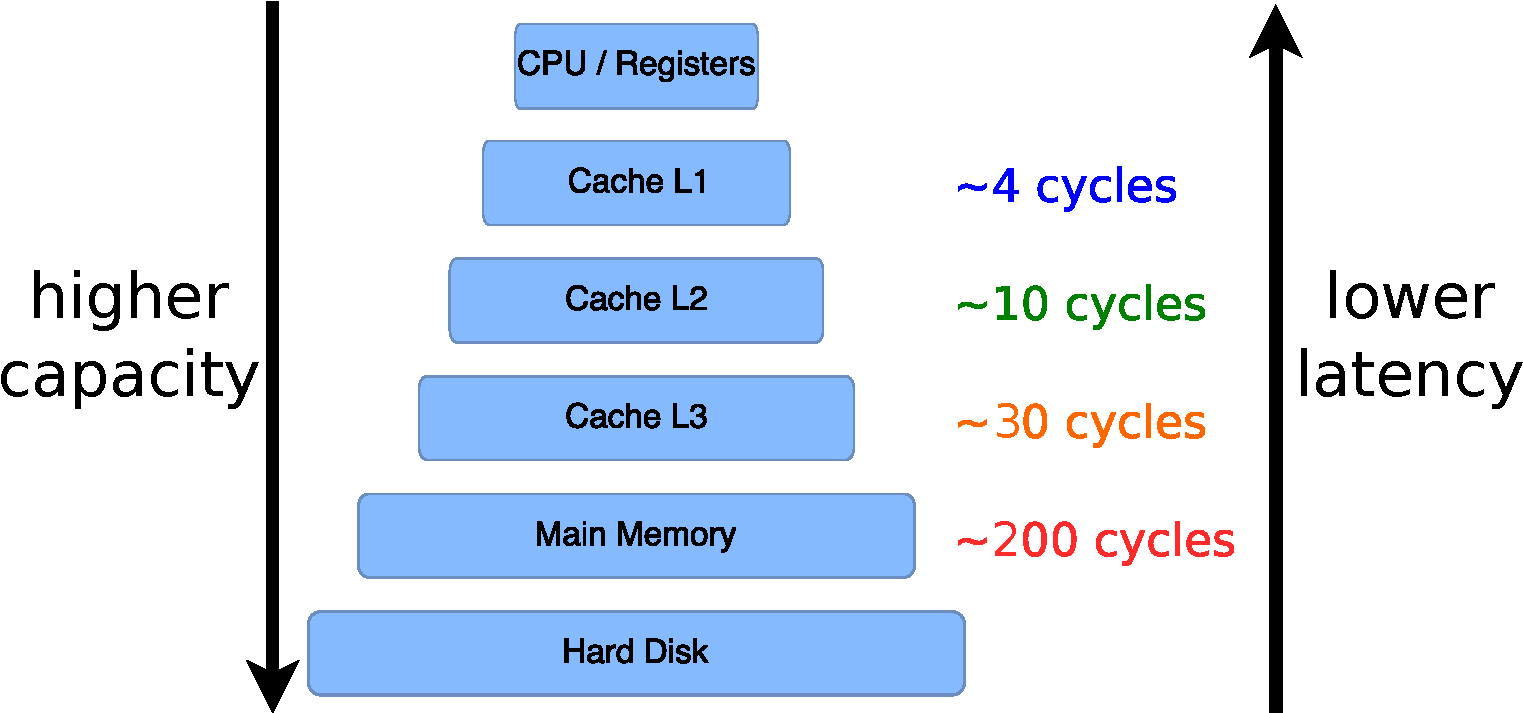
\includegraphics[width=0.7\linewidth]{img/tecnica/memoryHierarchy}
    % \caption{Hierarchy of memory present in modern computers. The hierarchy is compose by hard disk, main memory, three levels of cache and CPU registers. Adapted from~\cite{patterson2013computer}.}
    % \caption[Hierarquia de memória]{Hierarquia de memória presente em computadores modernos. A hierarquia é composta por disco rígido, memória principal, três níveis de cache e registradores. Adaptada de~\cite{patterson2013computer}.}
    \caption[Hierarquia de memória]{Hierarquia de memória presente em computadores modernos. Adaptada de~\citeonline{patterson2013computer}.}
    \label{fig:memoryHierarchy}
\end{figure}

A \textbf{localidade espacial} (\textit{spatial locality}) é uma propriedade importante dos sistemas hierárquicos de memória. Esta propriedade afirma que a probabilidade de acessar uma posição da memória é maior se uma posição próxima já foi referenciada~\cite{patterson2013computer}. O sistema de \textit{cache} explora esta propriedade armazenando os dados em blocos (\textit{cache blocks}). Assim, sempre que algum dado é acessado a partir da memória principal, ele é recuperado para a \textit{cache} juntamente com outros dados que estavam armazenados próximos a ele. Consequentemente, se os dados próximos forem acessados posteriormente, resultarão em \textit{cache hits}.


% cache arare ?
% cache oblivious ?

% \section{síntese física}
% \label{sec:conceitosFundamentaisSinteseFisic}
% % conceitos em Physical Design
% %     -- GCell
% %     -- skew (footnote)
% %     -- grid-graph


% \textit{\textbf{Clock Skew}} é a máxima diferença no tempo de chegada (\textit{arrival time}) do sinal de relógio entre todos os elementos sequenciais. Se $t(u,v)$ representa o atraso na chegada do sinal de relógio entre os elementos sequenciais $u$ e $v$, o \textit{skew} de uma rede de relógio $T$ é calculado segundo a Equação \ref{eq.skew}.
% \begin{equation} \label{eq.skew}
% 	 \displaystyle \operatorname{\textit{skew}(T)} = \max_{S_{i}, S_{j} \in S} | t(S_{0},S_{i})-t(S_{0},S_{j})|
% %	 \displaystyle \operatorname{\textit{skew}(T)} = \max_{i,j \in S} | at_i^L - at_j^L|
% \end{equation} 


\section{Ferramentas para avaliar o número de \textit{cache miss}}
\label{sec:ferramentasMiss}

%     PAPI (http://icl.cs.utk.edu/papi/)
%         executa na máquina hospedeira
%         instrumenta porções do código
%         somente arquitetura da maquina hospedeira
%         utiliza hardware counters
%         possibilita medr L1, L2 e L3 (instruções e dados)
   
A ferramenta \textit{Performance Application Programming Interface} (PAPI) \cite{papi} é desenvolvida pelo \textit{Innovative Computing Laboratory} da \textit{University of Tennessee}.
Esta ferramenta fornece ao programador uma interface para o uso de contadores de \textit{hardware} presentes nos processadores.
Ela permite estabelecer uma relação entre o desempenho do \textit{software} e os eventos do processador.
A instrumentação do código fonte é realizada por meio da inclusão da API da ferramenta PAPI e da inicialização de suas estruturas.
Com isso, é possível avaliar apenas uma porção do código fonte e retirar interferências indesejadas, como por exemplo aquelas oriundas das leituras de arquivos (\textit{parsing}).

\begin{table}[b]
\centering
\caption{Eventos presentes PAPI}
\label{tab:eventosPAPI}
\resizebox{\textwidth}{!}{%
\begin{tabular}{@{}llcl@{}}
\toprule
\multicolumn{1}{c}{Nome} & \multicolumn{1}{c}{Código} & Derivado & \multicolumn{1}{c}{Descrição}    \\ \midrule
PAPI\_L1\_DCM            & 0x80000000                 & Não      & Level 1 data cache misses        \\
PAPI\_L1\_ICM            & 0x80000001                 & Não      & Level 1 instruction cache misses \\
PAPI\_L1\_TCM            & 0x80000006                 & Sim      & Level 1 cache misses             \\
PAPI\_L2\_DCM            & 0x80000002                 & Sim      & Level 2 data cache misses        \\
PAPI\_L2\_ICM            & 0x80000003                 & Não      & Level 2 instruction cache misses \\
PAPI\_L2\_TCM            & 0x80000007                 & Não      & Level 2 cache misses             \\
PAPI\_L3\_TCM            & 0x80000008                 & Não      & Level 3 cache misses             \\
PAPI\_PRF\_DM            & 0x8000001c                 & Não      & Data prefetch cache misses       \\ \bottomrule
\end{tabular}%
}
\end{table}

A Tabela~\ref{tab:eventosPAPI} apresenta algum dos eventos que podem ser avaliados com a ferramenta PAPI e que estão disponíveis para a máquina utilizada nos experimentos deste trabalho, cuja configuração é descrita na Seção~\ref{sec:infraestrutura_experimental}.
Estes eventos variam de acordo com os contadores presentes em cada máquina e podem ser listados com o comando ``papi\_avail -a''.
Um evento pode estar diretamente disponível como um único contador, derivado usando uma combinação de contadores ou indisponível.
A terceira coluna indica se o evento utiliza ou não uma combinação de contadores de \textit{hardware}.

Devido ao fato de depender dos contadores da máquina hospedeira, uma análise que considere diferentes organizações de memória exige, necessariamente, a realização de experimentos em máquinas com características distintas, o que se constitui em dificuldade extra em termos de infraestrutura experimental.

%Uma limitação desta ferramenta, por depender dos contadores da máquina hospedeira, é o impedimento de simular diversas arquiteturas de memória e quantizar os ganhos para um determinado executável.

%     Perf (https://www.gnu.org/software/gperf/)
%         executa na máquina hospedeira
%         somente arquitetura da maquina hospedeira
%         utiliza hardware counters
%         somente medições na L1 e Last Level

%A ferramenta Perf: \textit{Linux profiling with performance counters} \cite{perf} é uma ferramenta de análise de desempenho do Linux. 
Perf (\textit{Linux profiling with performance counters} \cite{perf}) é uma ferramenta de análise de desempenho do Linux capaz de criar um perfil estatístico de todo o sistema (tanto o \textit{kernel} quanto o código do usuário) utilizando os contadores de \textit{hardware}. Portanto, esta ferramenta também é limitada pela arquitetura presente na máquina hospedeira.
Além disso, com Perf não é possível limitar-se a análise a somente parte do código fonte, uma vez que 
o relatório gerado somente realiza estatísticas no nível de funções do código fonte, não medindo as informações internas a elas (por linhas de código fonte).
Apesar de tais limitações, em 2012 dois engenheiros da IBM reconheceram Perf como sendo uma das ferramentas mais utilizadas no Linux \cite{perfIBM}.


%     Valgrind - cachegrind (http://valgrind.org/)
%         simula arquitetura (simulates how your program interacts with a machine's cache hierarch)
%         possibilita diversas arquiteturas
%         somente medições na L1 e Last Level

O \textit{framework} \textit{Valgrind} \cite{valgrind} possibilita a construção de ferramentas de análise dinâmica.
Existem ferramentas \textit{Valgrind} que podem detectar automaticamente muitos \textit{bugs} de gerenciamento de memória.
Dentre estas ferramentas, \textit{Cachegrind} \cite{cachegrind} possibilita a simulação da execução de um binário sobre diversas configurações de arquiteturas de \textit{cache}.
Sua execução é dada com o comando ``valgrind --tool=cachegrind prog'' onde ``prog'' representa o executável desejado.
A configuração da simulação permite definir o tamanho da memória \textit{cache}, sua associatividade, o tamanho de suas linhas e a política de escrita (por exemplo, quando um miss de escrita ocorre, o bloco escrito é colocado na \textit{cache} D1).
Tal flexibilidade permite a esta ferramenta simular uma infinidade de arquiteturas existentes ou até mesmo novas arquiteturas.
Porém, a simulação somente reporta resultados referentes ao primeiro e ao último nível da arquitetura de memória (L1 e LL respectivamente).

%     Intel VTune (https://software.intel.com/en-us/intel-vtune-amplifier-xe)
%         pago
%         precisa compilar o código com ICC

Já a ferramenta Intel VTune Amplifier \cite{intelVtune} possibilita uma análise entre múltiplas CPUs e utiliza os contadores de \textit{hardware}. 
Para utilizar esta ferramenta é preciso compilar a aplicação que será testada com o compilador ICC (Intel C++ Compiler) \cite{icc}.
% O ponto negativo desta ferramenta é que é preciso adquirir uma licença de \textit{software} para utiliza-la.
O ponto negativo desta ferramenta é o fato da licença de uso ser paga.



% \section{Ferramentas para medição do tempo de execução}
% \label{sec:ferramentasRuntime}

% %     -- std::chrono


